\section{Experiments}
\label{sec:experiments}
% \tk{order: CLEVR + baselines without TL, COG + baseline without TL, Feature Transfer-CLEVR/CoGenT, Temporal Transfer - COG, Reasoning Transfer - CLEVR/CoGenT, Reasoning Transfer-COG}

We implemented and trained our SAMNet model using MI-Prometheus~\cite{kornuta2018accelerating}, a framework based on PyTorch~\cite{paszke2017automatic}.
We evaluated the model on 
the CLEVR dataset~\cite{johnson2017clevr}, a diagnostic dataset for Image Question Answering and on the COG dataset~\cite{yang2018dataset}, a video reasoning~\cite{mogadala2019trends} dataset developed for the purpose of research on relational and temporal reasoning.
We briefly describe both datasets in the following two subsections.
In all experiments we used SAMNet using $k = 8$ reasoning steps and external memory with $N = 8$ slots, each storing an array of 128 floats. 
When working with all CLEVR/CoGenT variants we deactivated SAMNet's external memory and temporal-related modules as they are unnecessary while reasoning about static images.

We start with a sanity check of the performance of SAMNet in comparison with the selected SOTA baselines on both CLEVR and COG datasets without transfer learning.
The rest of the experiments follows the proposed taxonomy.
First, we investigate the feature transfer using the CLEVR-CoGenT variants, followed by the temporal transfer on the COG variants. Finally, we assess transfer reasoning capabilities on both datasets by regrouping and reorganizing classes of questions into new training and test splits.

\begin{table}[b!]
	\centering
	%\begin{adjustbox}{width=0.45\textwidth}
	\begin{tabular}{cccc}
		\toprule
		Variant	& Cubes	& Cylinders &	Spheres	\\
		\midrule
		CLEVR &  Any Color  & Any Color 	&	Any color  \\
		CoGenT-A &  Family A  & Family B 	&	Any color  \\
		CoGenT-B	&	Family B  &	Family A	&	Any color \\
		\bottomrule
	\end{tabular}
	%\end{adjustbox}
	\caption{Allowed feature combinations in the CoGenT-A and CoGenT-B variants of the CLEVR dataset.}%\vspace{2pts}
	\label{tab:cogent_conditions}
\end{table}

\begin{figure*}[t!]
	\centering
	\begin{subfigure}{\textwidth}
		\centering
		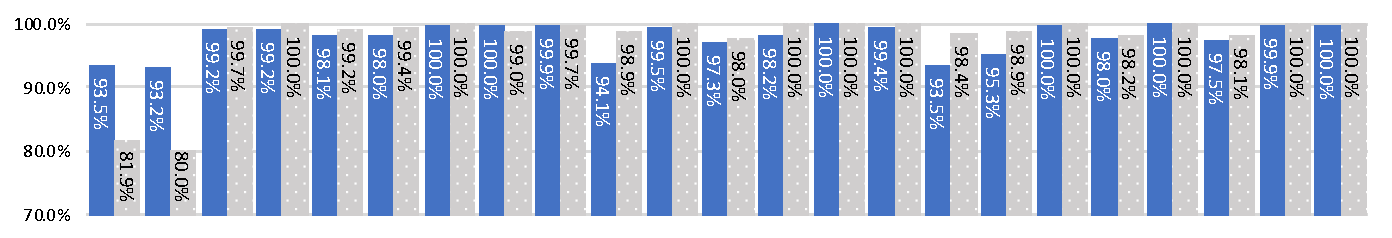
\includegraphics[width=0.9\textwidth]{../img/plots/cog_canonical_baseline_no_labels.pdf}
	\end{subfigure}%
	\newline
	\begin{subfigure}{\textwidth}
		\centering
		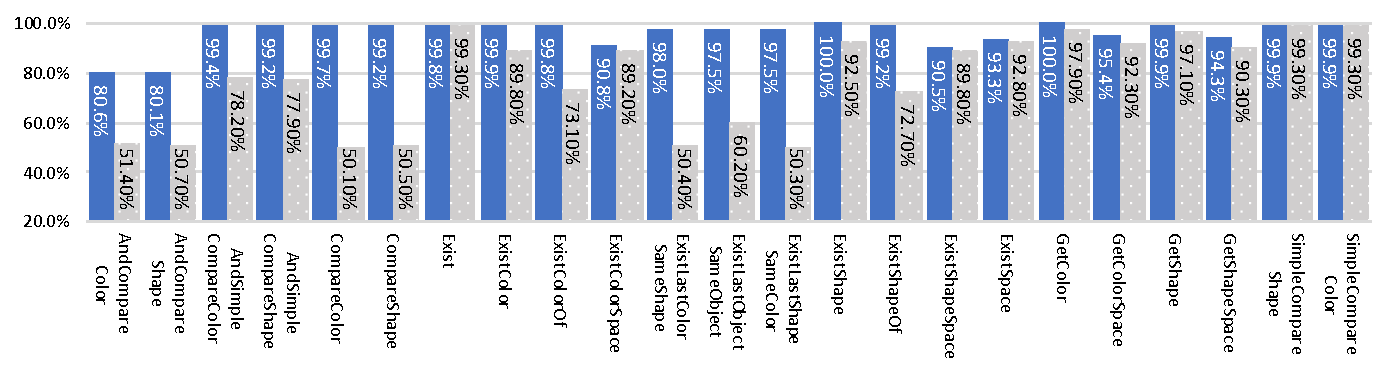
\includegraphics[width=0.9\textwidth]{../img/plots/cog_hard_baseline_labels.pdf}
	\end{subfigure}%
	\caption{Comparison of test set accuracies of SAMNet (blue) with original results achieved by the baseline model~\cite{yang2018dataset} (dotted gray) on Canonical (top) and Hard (bottom) variants of the COG dataset.}
	\label{fig:samnet_cog_detailed}
\end{figure*}

\subsection{Basic performance of SAMNet on CLEVR}
\label{sec:clevr-baseline-compare}
CLEVR images contain objects characterized by a set of attributes (shape, color, size and material), whereas the questions are grouped into 5 categories: \textit{Exist}, \textit{Count}, \textit{CompareInteger}, \textit{CompareAttribute}, \textit{QueryAttribute}.
The team behind the CLEVR dataset also introduced two CLEVR-CoGenT (Constrained Generalization Test) A and B variants, with varying combinations of color-shape attributes.
The colors are partitioned into two complementary families:
Gray, Blue, Brown and Yellow in Family A; and Red, Green, Purple, Cyan in Family B.
The cubes and cylinders take colors from complementary families in each variant with opposite configurations; the spheres can take any color in both varianrs (See~\cref{tab:cogent_conditions}).
As the input domain consist of the set of objects with all attribute values, both variants differ by their marginal distributions $P_S$ and $P_T$.

\begin{figure}[htbp]
	\centering
	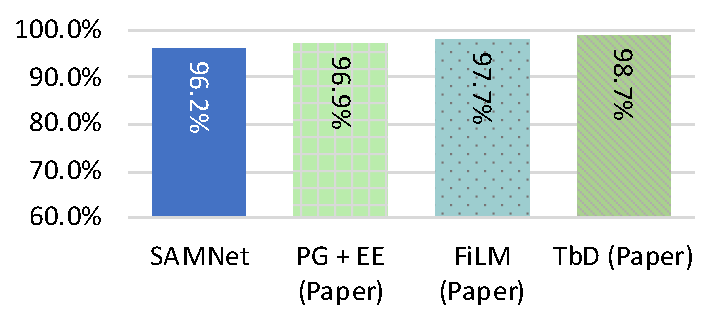
\includegraphics[width=0.8\columnwidth]{../img/plots/clevr_baselines.pdf}
	\caption{Comparison of SAMNet to baselines on CLEVR.}
	\label{fig:clevr_baselines}
\end{figure}

\cref{fig:clevr_baselines} presents accuracy achieved by SAMNet when compared to selected SOTA models, namely: Transparency by Design networks (TbD)~\cite{mascharka2018transparency}, Feature-wise Linear Modulation (FiLM)~\cite{perez2018film} and the Program Generator + Execution Engine (PG + EE)~\cite{johnson2017inferring}.
SAMNet reaches comparable 96.2\% accuracy, with TbD achieving the best score with 98.7\%.


\subsection{Basic performance of SAMNet on COG}
\label{sec:cog-baseline-compare}

COG dataset contains short videos, with the associated questions grouped into 23 categories~\footnote{Aside of categorical questions, COG also offers tasks expecting the model to point a particular object in the image (out of scope for this paper).}.
COG comes in two variants: the Canonical (easy) and Hard, differing mainly on the number of frames in the video, the maximum amount of look-back in frame history containing relevant information for reasoning, and the number of object distractors present in a given frame (see~\cref{tab:cog_variants}).
Since the number of task classes is large, we designed a 2-level hierarchy of task groups using the
description of tasks, as shown in~\cref{fig:task-groups}.

\begin{table}[ht]
	\centering
	\begin{tabular}{lccc}
		\toprule
		Variant	& Frames & History	& Distractors \\
		\midrule
		Canonical (Easy) & 4 & 3 & 1\\
		Hard  & 8 & 7 & 10\\
		\bottomrule
	\end{tabular}
	\caption{Details of the Canonical and Hard variants of COG.}
	\label{tab:cog_variants}
\end{table}


\begin{figure}[htbp]
	\centering
	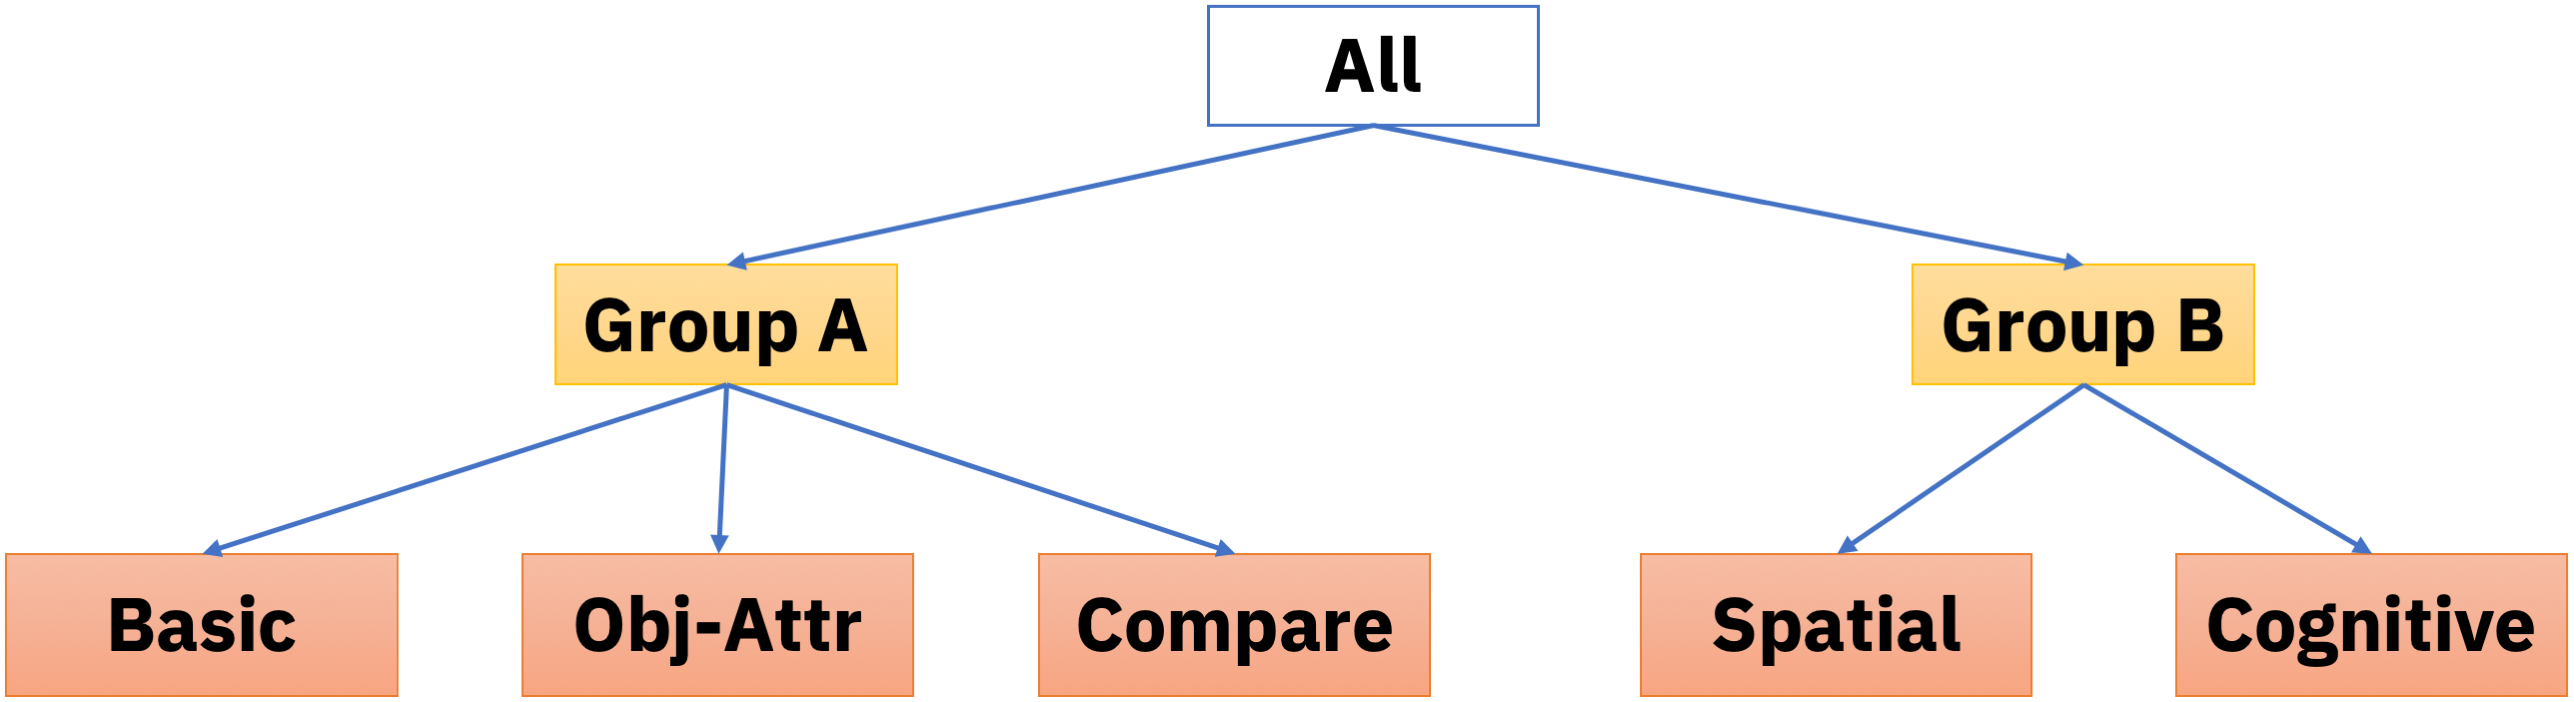
\includegraphics[width=\columnwidth]{../img/architecture/hierarchy}
	\caption{Hierarchy of Task Groups in the COG dataset.}
	\label{fig:task-groups}
\end{figure}



For groups at the lowest level, we chose the following task classes to be placed in those groups.
Below, substitute each of \textit{Shape} and \textit{Color} for  \uX{} to obtain the task class.
\begin{description}
	\compresslist
	\item[Basic:] \textit{Exist}\uX, \textit{Get}\uX{} and \textit{Exist};
	\item[Obj-Attr:] \emph{SimpleCompare}\uX{} and \textit{AndSimpleCompare}\uX;
	\item[Compare:] \textit{Compare}\uX,  \textit{AndCompare}\uX{} \& \textit{Exist}\uX\textit{Of};
	\item[Spatial:] \textit{ExistSpace}, \textit{Exist}\uX\textit{Space}, and \textit{Get}\uX\textit{Space};
	\item[Cognitive:] \textit{ExistLastColorSameShape}, \textit{ExistLastShapeSameColor} and \textit{ExistLastObjectSameObject}
\end{description}


We compared our results with the baseline model introduced in the same paper as the COG dataset~\cite{yang2018dataset}.
The most important results are highlighted in~\cref{fig:samnet_cog_detailed}; full comparison can be found in the supplementary material.

For the Canonical variant (top row), we achieve similar accuracies for the majority of tasks (with a total average accuracy of 98.0\%, compared to 97.6\% for the baseline model), with significant improvements (around 13 points) for \textit{AndCompare} tasks.
As these tasks focus on compositional questions referring to two objects, we hypothesize that our model achieves better accuracy due to its ability to selectively pick and store relevant objects from the past frames in its external memory.
For the Hard variant, we achieve a total average accuracy of 96.1\% compared to 80.1\% for the baseline model, demonstrating that our model can adapt to larger number of frames and distractors.
SAMNet improves upon the baseline model on all tasks, with improvements varying from 0.5 to more than 30 points, especially outperforming in the most complex (\textit{AndCompare}\uX, \textit{Compare}\uX) tasks.


\subsection{Feature transfer using CLEVR-CoGenT}
\label{sec:feature}

In order to quantify SAMNet feature transfer capabilities we used the CoGenT variants of CLEVR and performed a set of experiments, starting from training on CoGenT-A followed by:
an immediate test (zero-shot learning) to test split ot CoGenT-B; and fine-tuning for a single epoch on 30k samples from CoGenT-B before testing (following methodology used in~\cite{johnson2017inferring, mascharka2018transparency, perez2018film, marois2018transfer}).
In \cref{fig:CoGenT-B-results} we compare the achieved performance with the previously selected SOTA models. 
As sanity check we also provide accuracies achieved when: tested directly on CoGenT-A; and tested on CoGenT-A after fine-tuning on B.

\begin{figure}[htbp]
	\centering
	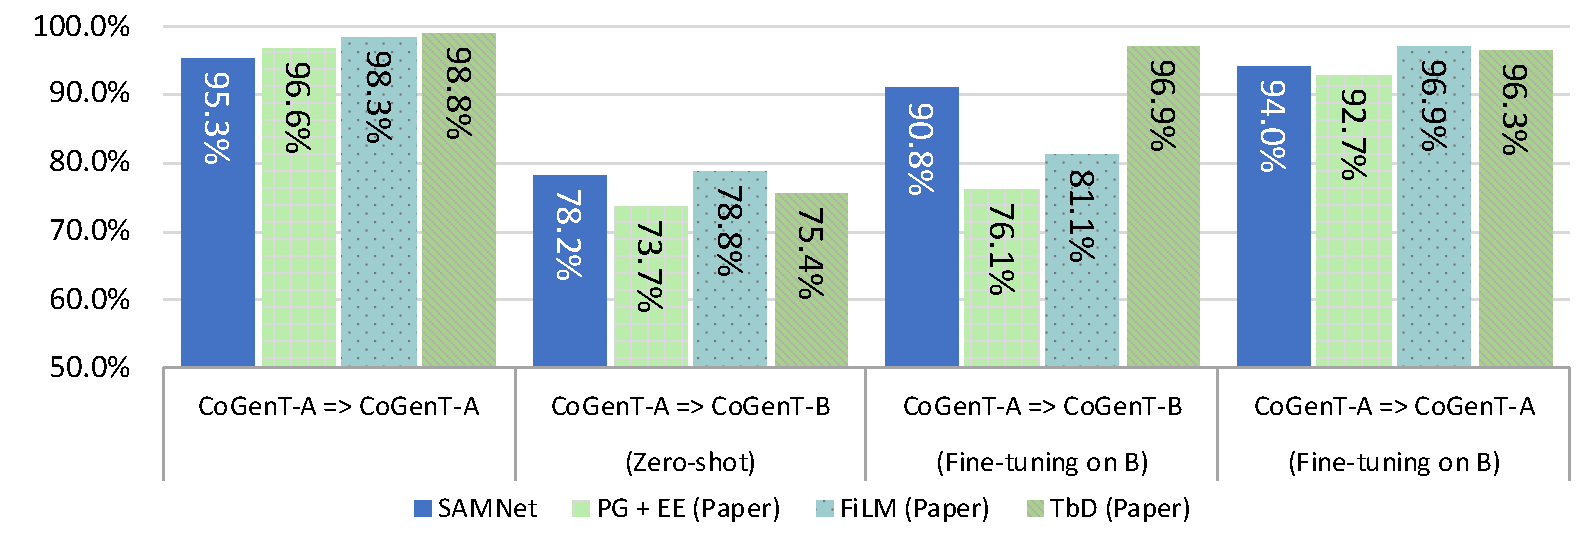
\includegraphics[width=\columnwidth]{../img/plots/cogent_feature_transfer_baselines.pdf}
	\caption{Feature transfer: test accuracties when transfering between the CoGenT-A and CoGenT-B variants.}
	\label{fig:CoGenT-B-results}
\end{figure}

When training and testing on CoGenT-A, SAMNet performs slightly worse than the other models, what is consistent with results on the basic CLEVR variant.
In the case of zero-shot transfer to CoGenT-B all models show relatively good performance (around 75 percent), still being a significant decrease of accuracy (by 17 points).
As expected, all models are able to recover performance when fine-tuned on CoGenT-B.
However, this process also results in degradation of performance on originally mastered CoGenT-A, with SAMNet and TbD showing clear capabilities to limit the impact of catastrophic forgetting.
This indicates that both SAMNet and TbD managed to develop and sustain (to some extent) representations of features when facing shift from one domain to the other.
Still, the drop in zero-shot transfer suggests that both struggle with disentanglement of shape and color features.

\subsection{Temporal transfer in COG}
\label{sec:temporal}

Temporal transfer tests the transfer learning ability concerning the frame sequence length, frame history required for reasoning, and the number of distracting objects.
Therefore, we train the models on the Canonical variant of COG dataset and test them on the Hard variant~(\cref{fig:samnet_cog_overall_transfer}).
As the original paper~\cite{yang2018dataset} didn't provided such experiments, we supplement the original accuracies (denoted as gray-dotted) with the ones achieved by the COG baseline model that we have obtained by running the original code (gray-striped) provided by the authors~\cite{yang2018implement}.

\begin{figure}[htbp]
	\centering
	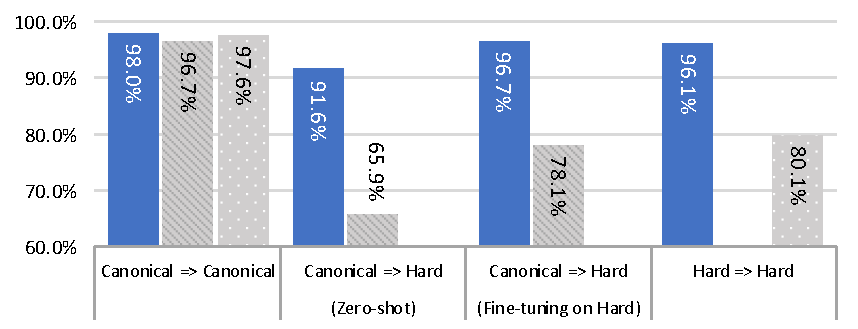
\includegraphics[width=\columnwidth]{../img/plots/cog_temporal_transfer_baselines.pdf}
	\caption{Temporal transfer capabilites of SAMNet (blue) and baseline models (gray -striped and -dotted) when moving from Canonical to Hard variants of the COG dataset.}
	\label{fig:samnet_cog_overall_transfer}
\end{figure}

The first column displays the aggregated scores when training and testing on the Canonical variant.
Similar scores of both base models (gray striped and dotted) underscore the reproducibility of the baseline model .
For both cases of zero-shot learning and fine-tuning using a single epoch, SAMNET significantly outperformed the baseline model, by 25 and 17 points respectively.
This might partially result from the frame-by-frame processing of videos executed by SAMNet by design, as opposed to the processing of aggregated frames performed by the baseline.
Interestingly, fine-tuning yields a mild boost of +0.6\% on the accuracy achieved by the model trained exclusively on the Hard variant.
This suggest that SAMNet managed to develop elementary skills (like good memory usage and attention on relevant entities) and successfully build on them when dealing with longer videos and more complex scenes.

%This suggest that it suffices to train SAMNet on simpler videos to enable learning of good memory usage and attention on relevant entities in order to achieve comparable, if not better, performance on longer video frames with more complex scenes.
